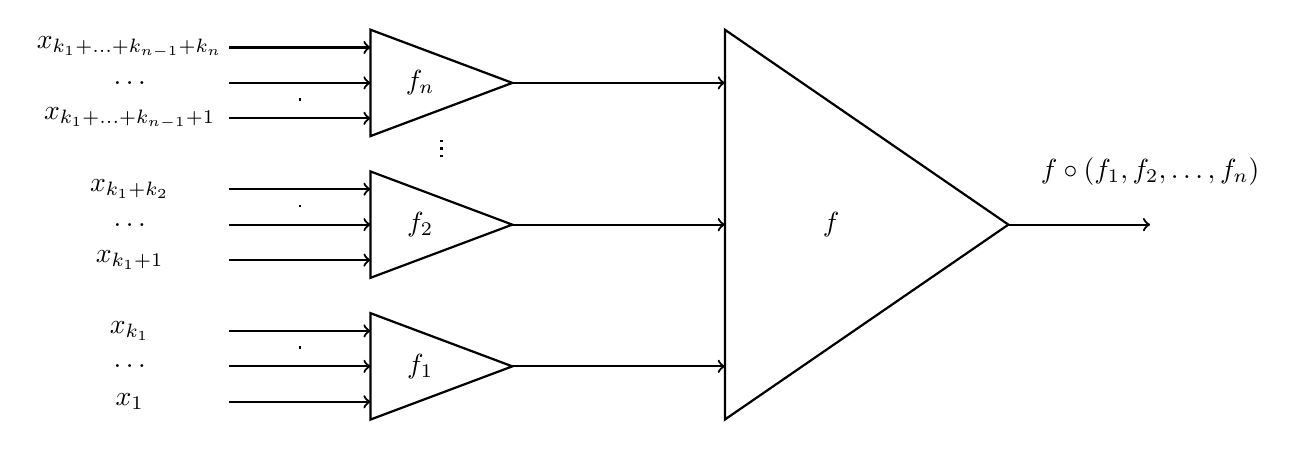
\begin{tikzpicture}[scale=0.9]
    % Main operation triangle
    \draw[thick, fill=white] (0,0) -- (0,5.5) -- (4,2.75) -- cycle;
    \node at (1.5,2.75) {$f$};

    % First sub-operation triangle
    \draw[thick, fill=white] (-5,0) -- (-5,1.5) -- (-3,0.75) -- cycle;
    \node at (-4.3,0.75) {$f_1$};

    % Second sub-operation triangle
    \draw[thick, fill=white] (-5,2) -- (-5,3.5) -- (-3,2.75) -- cycle;
    \node at (-4.3,2.75) {$f_2$};

    % Third sub-operation triangle (with dotted line indicating more)
    \draw[thick, fill=white] (-5,4) -- (-5,5.5) -- (-3,4.75) -- cycle;
    \node at (-4.3,4.75) {$f_n$};

    % Dotted line between second and third triangles
    \draw[dotted, thick] (-4,3.7) -- (-4,4);

    % Input arrows for first sub-operation
    \draw[->, thick] (-7,0.25) -- (-5,0.25);
    \draw[->, thick] (-7,0.75) -- (-5,0.75);
    \draw[->, thick] (-7,1.25) -- (-5,1.25);
    \node at (-8.4,0.25) {$x_1$};
    \node at (-8.4,0.75) {$\ldots$};
    \node at (-8.4,1.25) {$x_{k_1}$};

    % Input arrows for second sub-operation
    \draw[->, thick] (-7,2.25) -- (-5,2.25);
    \draw[->, thick] (-7,2.75) -- (-5,2.75);
    \draw[->, thick] (-7,3.25) -- (-5,3.25);
    \node at (-8.4,2.25) {$x_{k_1+1}$};
    \node at (-8.4,2.75) {$\ldots$};
    \node at (-8.4,3.25) {$x_{k_1+k_2}$};

    % Input arrows for third sub-operation
    \draw[->, thick] (-7,4.25) -- (-5,4.25);
    \draw[->, thick] (-7,4.75) -- (-5,4.75);
    \draw[->, thick] (-7,5.25) -- (-5,5.25);
    \node at (-8.4,4.25) {$x_{k_1+...+k_{n-1}+1}$};
    \node at (-8.4,4.75) {$\ldots$};
    \node at (-8.4,5.25) {$x_{k_1+...+k_{n-1}+k_n}$};

    % Connecting arrows from sub-operations to main operation
    \draw[->, thick] (-3,0.75) -- (0,0.75);
    \draw[->, thick] (-3,2.75) -- (0,2.75);
    \draw[->, thick] (-3,4.75) -- (0,4.75);

    % Output arrow
    \draw[->, thick] (4,2.75) -- (6,2.75);

    % Final output label
    \node at (6,3.5) {$f \circ (f_1, f_2, \ldots, f_n)$};

    % Dotted lines to indicate more inputs for each sub-operation
    \draw[dotted, thick] (-6,1) -- (-6,1.1);
    \draw[dotted, thick] (-6,3) -- (-6,3.1);
    \draw[dotted, thick] (-6,4.5) -- (-6,4.6);

\end{tikzpicture}